\documentclass[10pt,a4paper,english, twocolumn]{article}

\usepackage{graphicx} % This package draws images
\usepackage{hyperref} 
\usepackage{booktabs} % Essential for nice tabs (see https://people.inf.ethz.ch/markusp/teaching/guides/guide-tables.pdf)
\usepackage{multirow}

%page geometry
\usepackage[margin=0.8in]{geometry}

%encoding
%--------------------------------------
\usepackage[utf8]{inputenc} % input encoding
\usepackage[T1]{fontenc} % output encoding
%--------------------------------------

%French-specific commands
%--------------------------------------
\usepackage{babel}
\usepackage[autolanguage]{numprint}
%--------------------------------------

\usepackage{mathtools}
\usepackage{amsmath}
\usepackage{amssymb}

\addto\captionsenglish{% Replace "english" with the language you use
  \renewcommand{\contentsname}%
    {Table of contents}%
}

\usepackage{enumitem}

\usepackage[ruled]{algorithm2e}
\usepackage{parskip}
\usepackage{indentfirst}
\setlength{\parindent}{10pt}

\usepackage{subcaption}
\usepackage{caption}
\DeclareCaptionType{equ}[][]
\captionsetup[equ]{labelformat=empty}

\setcounter{secnumdepth}{2}
\setcounter{tocdepth}{2}

\title{\textbf{GPU-efficient and compressed representation of
implicit surfaces for real-time rendering} \\ INF515}
\author{Marius Debussche, \href{mailto:marius.debussche@polytechnique.edu}{marius.debussche@polytechnique.edu} \\ Clément Jambon, \href{mailto:clement.jambon@polytechnique.edu}{clement.jambon@polytechnique.edu} \\ Supervised by Tamy Boubekeur}

\begin{document}

\maketitle

\section{Introduction and motivations}
Signed distance functions (SDFs) provide a nice framework to represent and render complex 3D shapes. More precisely, in 3-dimensional spaces, they are defined as the distance of a point $x\in\mathbb{R}^3$ to a surface $\mathcal{S}$ and extended with a \textit{plus} or \textit{minus} depending on whether $x$ is outside or inside the surface. The main advantage of this representation lies in the representation of the related surface which can be defined with an "infinite" resolution, for example implicitely as the zero level-set of a continuous function $f:\mathbb{R}^3\to\mathbb{R}$ i.e $\mathcal{S}=\{x\in\mathbb{R}^3, f(x)=0\}$. Moreover, through this representation, such surfaces can easily be manipulated as primitives with fusion, addition, extrusion or more complex operations and aranged in practical datastructures such as \textit{CSG Trees} and used directly by artists (see for example MagicaCSG\footnote{\url{https://ephtracy.github.io/index.html?page=magicacsg}}, Clayxels\footnote{\url{https://andrea-intg.itch.io/clayxels}} or Adobe's Medium\footnote{\url{https://www.adobe.com/products/medium.html}}).

When represented as SDFs, implicit surfaces can be rendered with rasterization by deriving a mesh through marching cubes for example or thanks to ray tracing techniques such as \textit{Sphere Tracing} introduced by Hart in \cite{Hart1996SphereTA}. We chose to focus on the latter because, by casting rays for each pixel or so, they fully leverage the multiresolution caracteristics and smooth properties of the surfaces. Indeed, with a few dozens of iterations, we can reach the surface and knowing its equation (or by approximating its local aspect), we can infer the normal to the intersecting point of the ray and recast other rays in the scene.

\section{Preliminary works}
As a first preliminary work, we decided to implement a full sphere tracing pipeline in \textit{OpenGL}. To do so, we chose a few primitives (e.g. sphere, cube, etc.) and wrote the full ray casting algorithm in the fragment shader of the bounding box of our primitive.

\begin{figure}
    \begin{subfigure}{.5\linewidth}
        \centering
        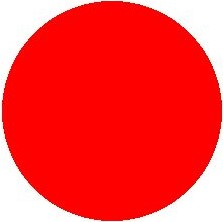
\includegraphics[width=.9\linewidth]{figures/ray_marching.JPG}
        \caption{without Phong shading}
        \label{sfig:sphere-tracing1}
    \end{subfigure}%
    \begin{subfigure}{.5\linewidth}
        \centering
        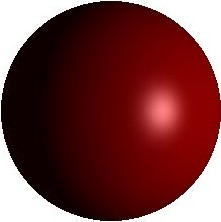
\includegraphics[width=.9\linewidth]{figures/ray_marching_phong.JPG}
        \caption{with Phong shading}
        \label{sfig:sphere-tracing2}
    \end{subfigure}
    \caption{SDF-based ray tracing of a sphere}
    \label{fig:sphere-tracing}
\end{figure}

As can be seen on image \ref{fig:sphere-tracing}, the obtained resolution is perfect and implies no artifacts as would be observed in conventional rasterization pipelines with a mesh of a sphere. More interestingly, with only a few additional lines of code in the fragment shader, we can recast a ray in the direction of a point source of light and perform Phong shading as shown in figure \ref{sfig:sphere-tracing2}.

However, we quickly faced a major hindrance in our exploration of SDF rendering. As they are run on the GPU, fragment shaders have strong constraints on the \textit{uniform} values that can be shared and updated between the "client", namely the CPU processing all the transformations of the scene and its inputs, and the "server", namely the GPU whose behaviour is controlled by shaders that, being executed in a very parallelized fashion, have a very restrictive way of exchanging information. More precisely, if we want to add reflections of other objects, shadows induced by various obstructing objects, take into account multiple reflexions to render soft shadows or add a growing number of lights in the scene, we need to pass all these information to the context of the shader which becomes clearly intractable as the scene grows in complexity. As a consequence, except for single shot and handcrafted scenes as can be found on \textit{Shadertoy}\footnote{\url{https://www.shadertoy.com/}}, this approach does not scale to a modular and generic editing tool as we envisioned to do.

Following a talk given by Sebastian Aaltonen at the Advanced Graphics Techniques Tutorial of GDC 2018 and entitled \textit{GPU-Based Clay Simulation and Ray-Tracing Tech in 'Claybook'}\footnote{\url{https://www.gdcvault.com/play/1025316/Advanced-Graphics-Techniques-Tutorial-GPU}}, we decided to turn to discretized versions of SDFs represented as volume textures (i.e 3D textures) and generated in \textit{compute shaders}.

\textit{Compute shaders} are not part of the regular rendering pipeline but allow to perform arbitrary operations on the GPU, for example generating textures on the fly in the GPU. More interestingly, \textit{compute shader} jobs are dispatched according to cartesian coordinates such as $x$, $y$ and $z$ and are thus, if properly designed, particularly suited to the task of handling volume textures. Nevertheless, a major constraint due to the GPU architecture is the notion of \textit{shared memory} and \textit{cache misses} that requires to devise proper workaround and heuristics. In his talk, Sebastian Aaltonen describes how he and his teammates generate a SDF texture from a set of predefined "brushes" (similar to primitives) and operations on such instanciated brushes (e.g.\ union, morphing, etc).

In order to get our hands with these notions, we decided to implement our own SDF sampling strategy and resulting rendering pipeline. To this extent, we, once again, decided to sample the SDF of simple primitives such as the sphere on a limited amount of bits. More precisely, following Aaltonen's work, we chose to encode the full SDF in samples of $8$ bits and according to a regular 3D grid bounding the primitive. This challenged us in the sense that we needed to properly discretize the sampled values of the distance field and the resolution needed to be wisely chosen. As can be seen in figure \ref{fig:sampled-sphere}, finer sampling resolutions of the SDF give finer visual renderings of the sphere.

\begin{figure}
    \begin{subfigure}{.3\linewidth}
        \centering
        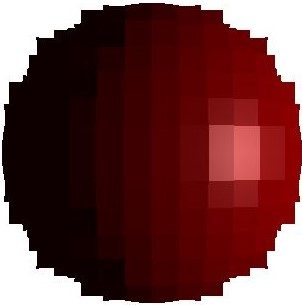
\includegraphics[width=.9\linewidth]{figures/discretized_sdf_32.JPG}
        \caption{$32^3$}
        \label{sfig:sampled-sphere1}
    \end{subfigure}
    \begin{subfigure}{.3\linewidth}
        \centering
        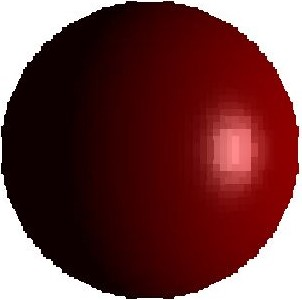
\includegraphics[width=.9\linewidth]{figures/discretized_sdf_128.JPG}
        \caption{$128^3$}
        \label{sfig:sampled-sphere2}
    \end{subfigure}
    \begin{subfigure}{.3\linewidth}
        \centering
        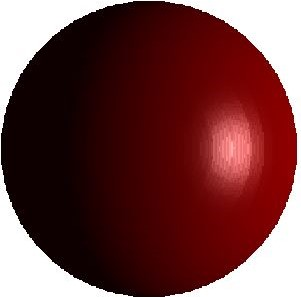
\includegraphics[width=.9\linewidth]{figures/discretized_sdf_512.JPG}
        \caption{$512^3$}
        \label{sfig:sampled-sphere3}
    \end{subfigure}
    \caption{Ray traced rendering of a sampled SDF of a sphere with increasing texture resolution.}
    \label{fig:sampled-sphere}
\end{figure}

As we can easily infer, the problem lies at the boundary of the sphere where the resolution of the sampled sphere is not precise enough to take into account the local structure of the corresponding surface. This challenge does not only concern the signed distance field itself but also the normals if we choose to encode them in a texture (as Sebastian Aaltonen did for \textit{Claybook}) This brought us to consider more advanced methods to sample the signed distance field and invited us to divide our work in two directions :
\begin{description}
    \item[Marius Debussche] $ $ \\
    a more practical approach of dynamically generating a SDF-based scene as the result of operations on a series of input "brushes", namely primitives and updating it in \textit{compute shaders} as the viewport moves in the scene and the scene changes following inputs from the user and pre-computed behaviours (e.g. physics).
    \item[Clément Jambon] $ $ \\
    a more theoretical approach of encoding and sampling the SDF suited to the GPU architecture and providing sufficient details at different resolutions (see section \ref{sec:representing-sdf} for currently considered directions) thus trying to avoid the artifacts shown in figure \ref{fig:sampled-sphere}.
\end{description}

\section{Representing SDFs: state-of-the-art and future directions}
\label{sec:representing-sdf}

As mentioned before, uniformly sampling SDFs as well as storing its scalar (as well as normal vectorial) values imply strong memory usage while not taking into account the structural aspect of the surface in the sampling strategy. To address, such issues, several approaches have been proposed.

\textit{Adaptively sampled distance fields} have been introduced in \cite{10.1145/344779.344899} and use octree datastructures to sample the signed distance field at multiple resolutions where more precision is required. The SDF can then be estimated by trilinear interpolation on the finest voxel surrounding the queried sample point. The issue with this octree datastructure is that updating the SDF as well sampling a value from this representation requires to access parts of memory that might be very distant from one another, thus triggering consuming cash misses that may slow dramatically the rendering process.

\textit{Hash-based} methods have been introduced in \cite{10.1145/2508363.2508374}, for example. These methods are quite efficient but tailored for \textit{voxel-based} rendering and not ray tracing where we are required to be able to sample the signed distance field everywhere in the accessible space. Some \textit{volumetric-based} representations such as \textit{GigaVoxels}\cite{crassin:inria-00345899} provide interesting schemes that we could get inspiration from.

As of today, we have identified two directions that we would like to explore in the following weeks to represent SDFs in compressed and adaptative ways. The first one, sparse coding through dictionary-based representations, is presented in paragraph \ref{ssec:dictionary-sdf} and relies on techniques that have proven to be very effective in other areas of Computer Graphics. The second one, neural local representations of distant fields, is introduced in paragraph \ref{ssec:neural-sdf} and finds its inspiration from very recent works in neural representation learning.

\subsection{Dictionary-based sampling of SDFs}
\label{ssec:dictionary-sdf}

Sparse coding and dictionary based structures have already proven to be very useful in other fields of computer graphics including 3D Modeling as presented in \cite{Lescoat:2018:3DDictSTAR}. However, to our knowledge, their extension for GPU-based rendering of signed distance field has not been tested yet. This motivates us to head towards this direction.

More precisely, at \textit{High Performance Programming 2021}, Kersten Schuster presented his work \cite{10.2312:hpg.20211284} on the compression and rendering of textured point clouds via sparse coding. The main idea behind the paper is to render splat textures of the point cloud as  sparse codings of a learned dictionary, namely a linear combination of a small number of atoms in the dictionary as given in equation \ref{eq:sparse-coding}. This dictionary-based scheme is achieved by concurrently learning the dictionary using the k-SVD algorithm introduced in \cite{1710377} and deriving the sparse coding of each splat thanks to \textit{Orthogonal Matching Pursuit}.

\begin{equ}[!ht]
    \begin{equation}
        y_i = \sum_{k=1}^{K_i}x_{i, k}d_{i, k}
      \label{eq:sparse-coding}
    \end{equation}
  \caption{where $d_i$ is a sample from the dictionary and $K_i$ satisfies $K_i\leq K$}
  \end{equ}

In this project, we would like to extend this method to volumetric SDF representations. To do so, we intend to create a coarse \textit{Sparse Voxel Octree} (SVO) with a small maximum depth where each end voxel in the tree (i.e. a voxel that has no children at lower levels) could be represented as a sparse coding of a pretrained dictionary of 3D volumetric textures that could act as samples of the SDFs themselves. This structure would be particularly interesting as it would allow to edit some parts of the volume without having, in practice, to recompute all the values of the decomposition every time for all the voxels of the octree. Indeed, as sphere tracing relies on suitably selected steps along the cast ray. If the structure of the scene changes sufficiently away from the updated voxels, it would not affect the ray casting strategy up to a few marching steps. Moreover, storing the SDF values inside a texture would allow for fast and efficient sampling while avoiding too much cache misses. The proposed strategy is illustrated in figure \ref{fig:sparse-coding-sdf}.

\begin{figure*}[h]
    \centering
    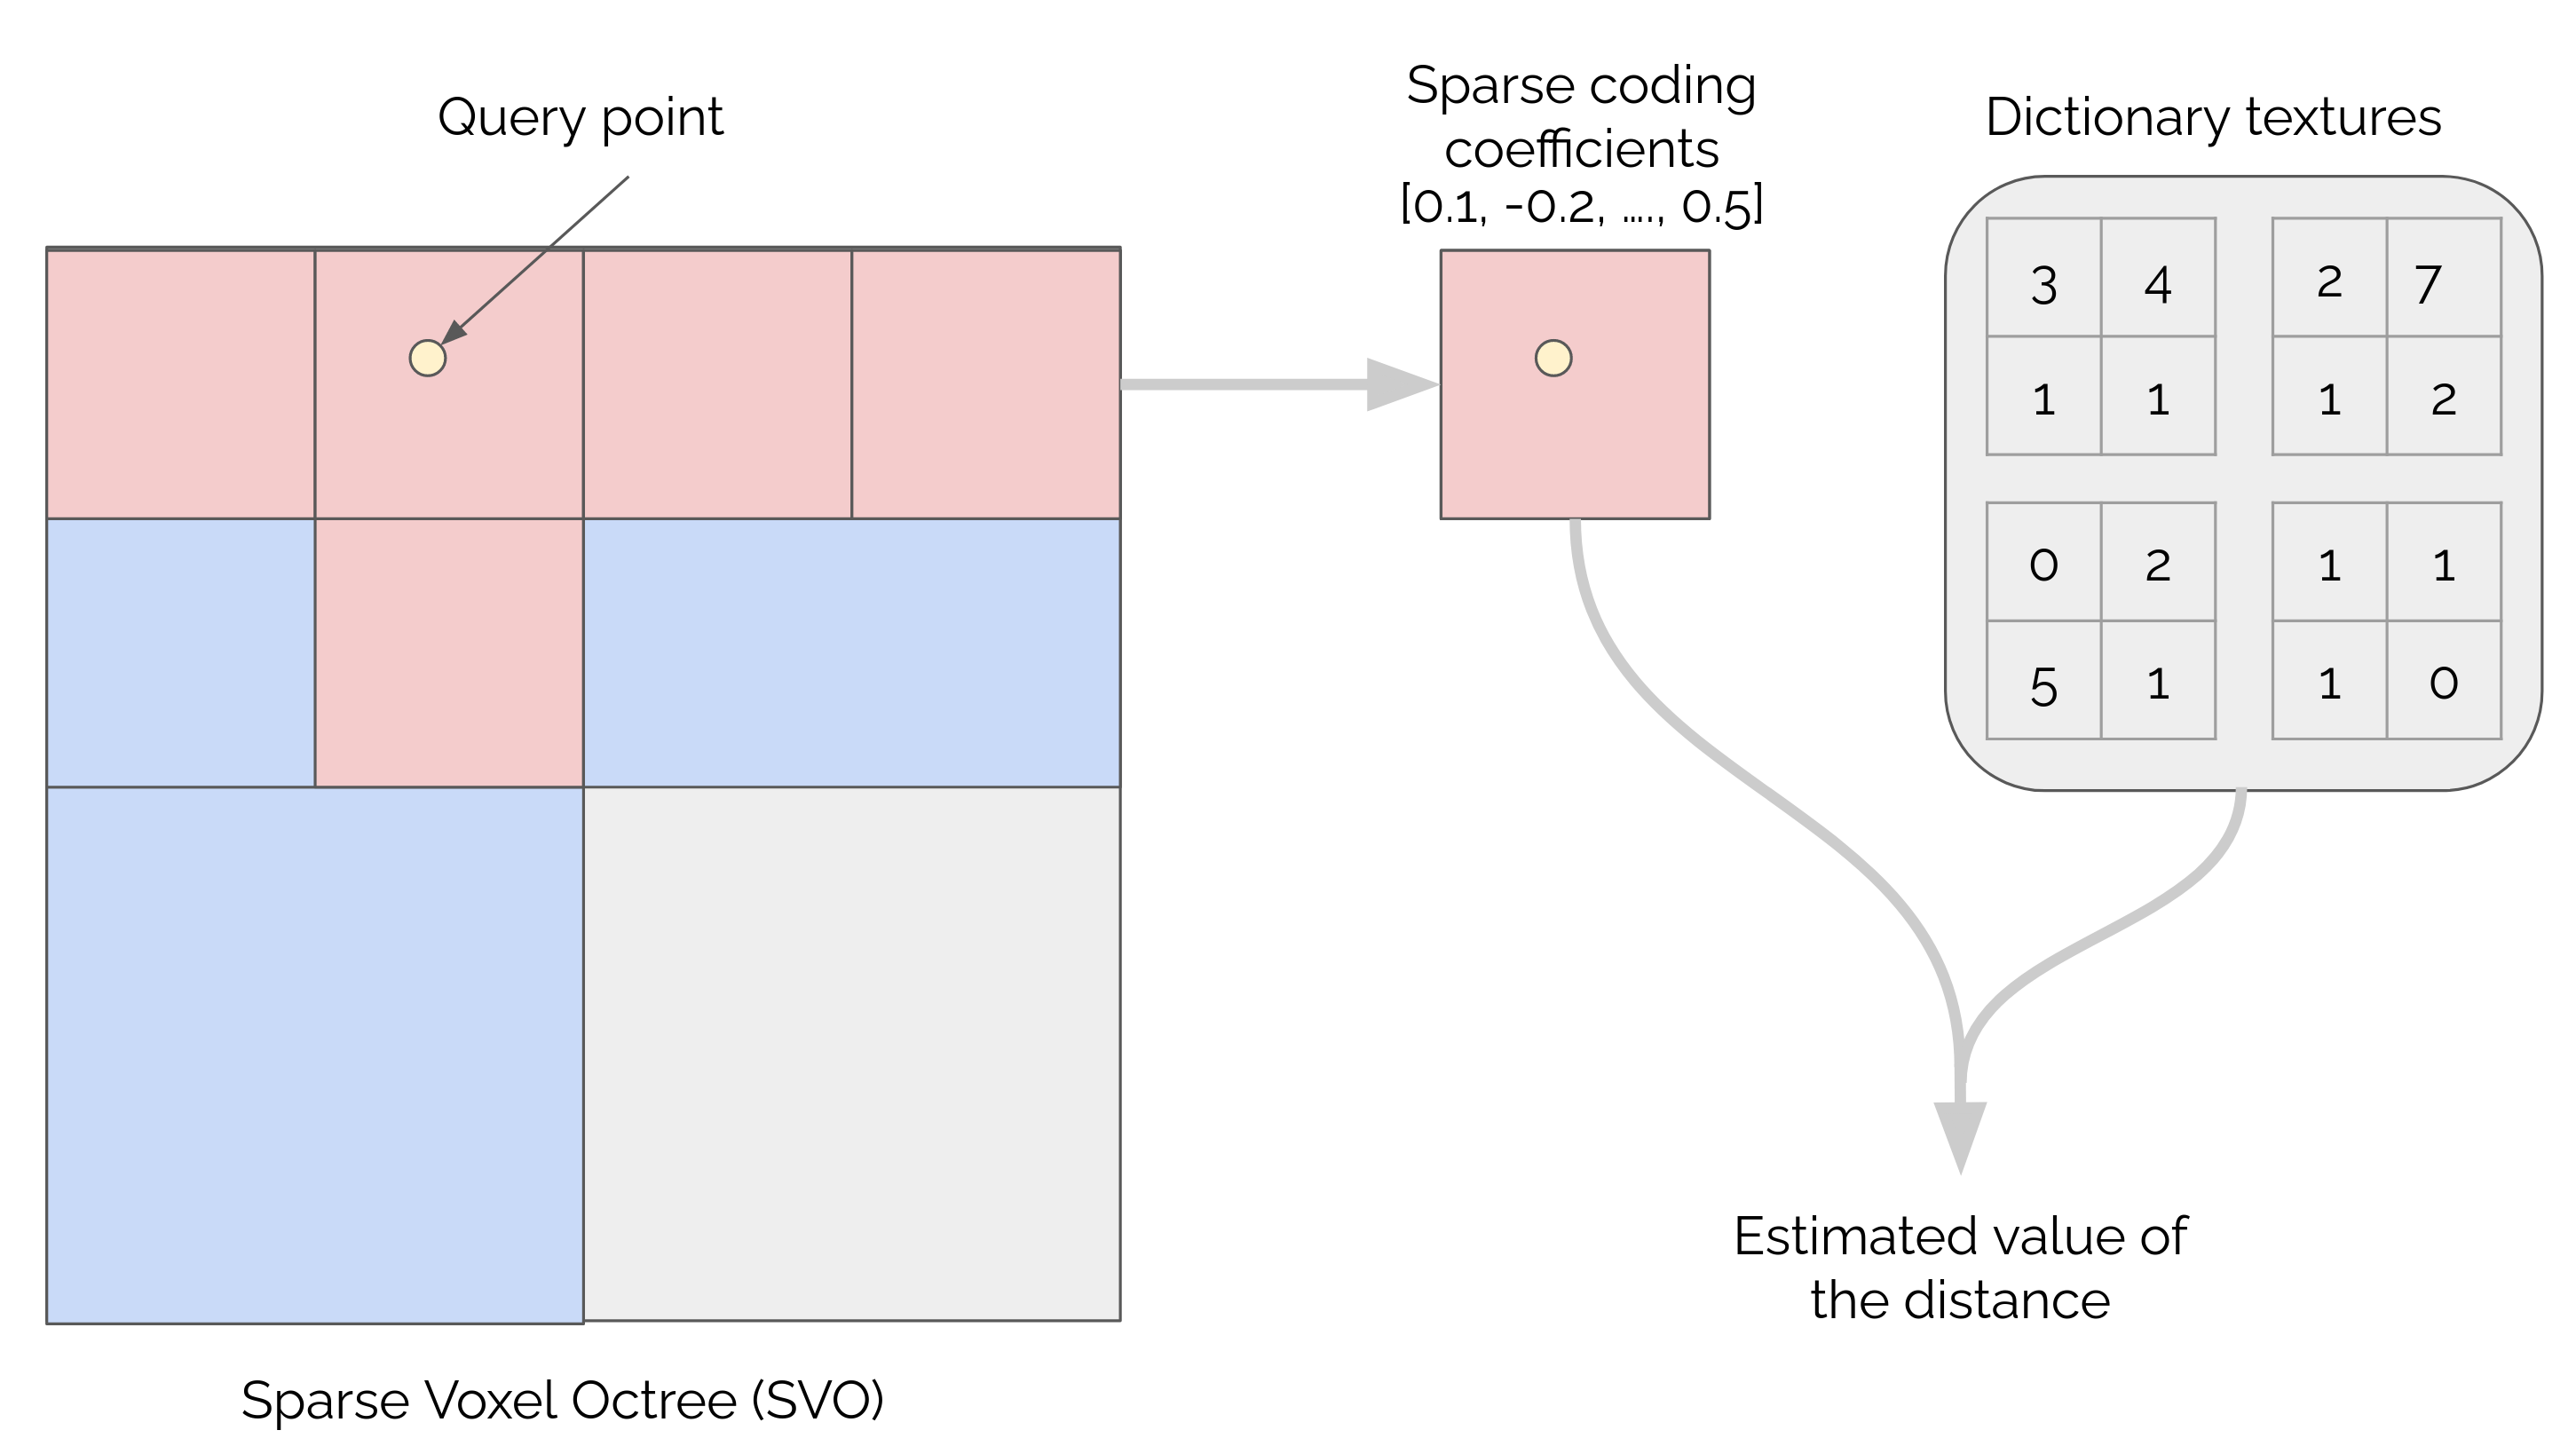
\includegraphics[width=0.8\textwidth]{figures/sparse-coding-sdf.png}
    \caption{Proposed dictionary-based representation of the SDF}
    \label{fig:sparse-coding-sdf}
\end{figure*}

\subsection{Neural representations of SDFs}
\label{ssec:neural-sdf}
Recently, they have been a lot of attempts to represent SDFs as neural networks. For example, \textit{DeepSDF} introduced in \cite{Park_2019_CVPR} proposes to represent a SDF as a global learned neural network. However, in order to capture the full complexity and details of the scene, the architecture of the network must be sufficiently large and rely on a large amount of parameters. As a consequence, inference on such a network is demanding and, as such, cannot be used for realtime rendering.

To address this issue, \cite{takikawa2021nglod} recently proposed to encode SDFs as latent representations learned by a small fixed neural network, namely a MLP with a single hidden layer of size $128$. These learned vectors are stored in a \textit{Sparse Voxel Octree} (SVO) and the SDF is sampled by summing the contributions of the features associated to each voxel across each level of the (SVO), applying trilinear interpolation in the sum and decoding it thanks to the aforementioned MLP.

As part of this project, we would like to implement a similar solution with a MLP that can be evaluated directly in a \textit{shader}. Moreover, as the scene faces radical changes, we would like to try and dynamically update the parameters of the decoding MLP and test the obtained result against existing solutions.

\section{Generating SDFs: roadmap}



\addcontentsline{toc}{section}{References}
\bibliographystyle{plain}
\bibliography{biblio}

\end{document}
